% Drawing 154/09-2 -- folder 154, batch 09, archive page 162 (PDF page 163).
% Transcription: page de dessins sans texte. À gauche, deux disques accolés en huit, bordés de vert clair, traversés de pseudo-droites rouges, secteurs coloriés en jaune ; une double flèche noire relie un point du bord du disque supérieur à un point du disque inférieur. Au milieu, un disque dont une moitié du bord est vert foncé et l'autre vert clair, traversé de pseudo-droites rouges ; au bord, des numéros $0$, $1$, $2$, $3$, $4$, $5$ d'un côté et $0'$, $1'$, $3'$, $4'$, $5'$ de l'autre, les deux sommets opposés (marqués $0$, $1$ et $0$, $1'$) coupés d'un trait bleu. Au-dessous, un rectangle arrondi bordé de vert clair et de tirets rouges, traversé de pseudo-droites rouges, une ligne médiane vert foncé, deux traits bleus sur les côtés. À droite, au crayon, un cercle traversé d'un diamètre, avec au bord les marques $\alpha$ (deux fois), $1$, $1'$, $2'$, $3'$, $4'$, $5'$, $3$, $4$, $5$
% Kind: figure of eight of two disks with arrangements; disk with numbered rim; elongated disk with bands; pencil disk with numbers. Method 2 (schematic redraw from the facsimile). Status: partial.
% Notes: Page of drawings without text, read from the page view. Left, two disks glued in a figure of eight, bordered in light green, crossed by red pseudolines, sectors coloured yellow (drawn as wedges); a black double arrow joins a point of the rim of the upper disk to a point of the lower. In the middle, a disk with a light and dark green rim, red pseudolines, its rim points numbered 1 ... 5 and 1' ... 5' (numbers not reproduced), blue marks at top and bottom; below it an elongated disk with dotted red rim, two blue marks at the sides, red strands and a dark green band. Right, a pencil disk with numbered rim points (1' ... 5', placed approximately). Strands schematic. Still differs from the facsimile: In the middle, a disk with a light and dark green rim, red pseudolines, its rim points numbered 1 ... 5 and 1' ... 5' (numbers not reproduced), blue marks at top and bottom; below it an elongated disk with dotted red rim, two blue marks at the sides, red strands and a dark green band. Right, a pencil disk with numbered rim points (1' ... 5', placed approximately). Strands schematic. 6 coloured or hatched triangle(s) are placed schematically and are not bounded by the strands that bound them on the page (2 now attached exactly).
% Coordinates: 1 unit = 1 mm = 1/100 of the crop width (bbox in page fractions: [0.202, 0.124, 0.937, 0.46]).
% Redrawn by Claude (claude-opus-5-5), issue #73, 2026-11-07; not checked by a human; not compiled (no TeX in the session).
% Revised by Claude (claude-opus-5-5) 2026-11-09 (issue #128) after Michel's check: vertices snapped to exact intersections (drawn points on their lines, meeting ends on the stroke they meet, near-concurrent lines through one computed point, curve ends on their rim); labels at \small as in folder 80 batch 3. Status: partial.
% Rights: reproduces part of the work -- behind RENDER_TRANSCRIPTS, never published by itself.
\documentclass[tikz,border=3pt]{standalone}
\usepackage{amsmath,amssymb}
\usetikzlibrary{patterns,arrows.meta}
\tikzset{Or/.style={orange!90!black}, Ye/.style={yellow!80!orange}, Lg/.style={green!60!black!70}, Dg/.style={green!45!black}, Br/.style={brown!80!black}, Rd/.style={red!85!black}, Bl/.style={blue!70!black}, Gy/.style={black!40}, pencil/.style={black!45}, struck/.style={black!35}, mark/.style={circle,draw,inner sep=1.3pt}, pt/.style={circle,fill,inner sep=0.9pt}, opt/.style={circle,draw,fill=white,inner sep=1.1pt}}
\begin{document}
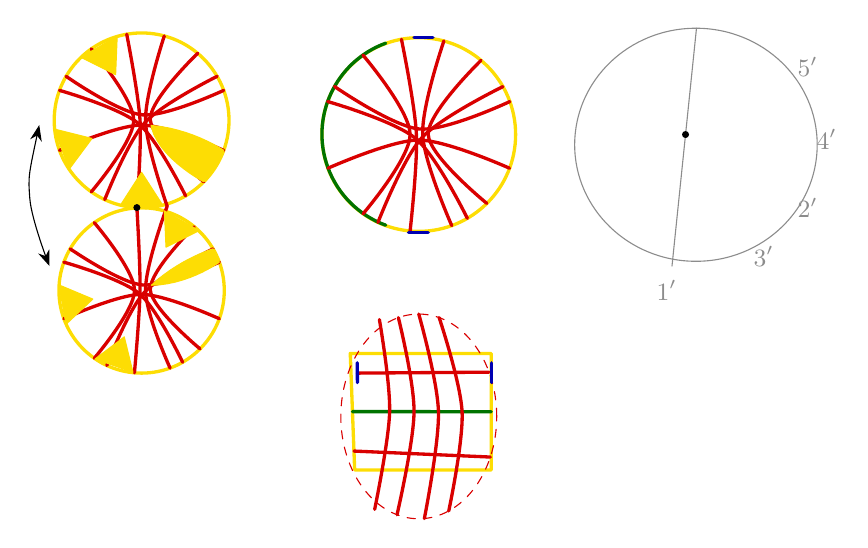
\begin{tikzpicture}[x=1mm,y=1mm,line cap=round,line join=round,font=\scriptsize]
\draw[Ye,very thick] (14.2,-13.6) circle[radius=11.1];
\draw[Ye,very thick] (14.2,-35.2) circle[radius=10.5];
\draw[Rd,very thick] plot[smooth, tension=0.55] coordinates {(12.31,-2.66) (14,-13.6) (13.6,-24.68)};
\draw[Rd,very thick] plot[smooth, tension=0.55] coordinates {(17.08,-2.88) (14.7,-13.6) (17.45,-24.5)};
\draw[Rd,very thick] plot[smooth, tension=0.55] coordinates {(7.81,-4.52) (13.2,-13.6) (7.81,-22.68)};
\draw[Rd,very thick] plot[smooth, tension=0.55] coordinates {(21.32,-5.08) (15.3,-13.5) (22.1,-21.4)};
\draw[Rd,very thick] plot[smooth, tension=0.55] coordinates {(4.61,-8.01) (14.3,-12.9) (24.63,-9.79)};
\draw[Rd,very thick] plot[smooth, tension=0.55] coordinates {(3.77,-17.41) (14.2,-14.2) (24.63,-17.41)};
\draw[Rd,very thick] plot[smooth, tension=0.55] coordinates {(23.79,-8.01) (14.6,-13.9) (9.52,-23.66)};
\draw[Rd,very thick] plot[smooth, tension=0.55] coordinates {(3.77,-9.79) (13.8,-14) (19.79,-23.19)};
\draw[Rd,very thick] plot[smooth, tension=0.55] coordinates {(13.6,-24.68) (14,-35.2) (13.29,-45.66)};
\draw[Rd,very thick] plot[smooth, tension=0.55] coordinates {(17.45,-24.5) (14.7,-35.2) (17.82,-45.06)};
\draw[Rd,very thick] plot[smooth, tension=0.55] coordinates {(8.19,-26.59) (13.3,-35.2) (8.19,-43.81)};
\draw[Rd,very thick] plot[smooth, tension=0.55] coordinates {(20.89,-27.11) (15.3,-35.1) (21.62,-42.62)};
\draw[Rd,very thick] plot[smooth, tension=0.55] coordinates {(5.13,-29.92) (14.3,-34.5) (24.07,-31.61)};
\draw[Rd,very thick] plot[smooth, tension=0.55] coordinates {(4.33,-38.79) (14.2,-35.7) (24.07,-38.79)};
\draw[Rd,very thick] plot[smooth, tension=0.55] coordinates {(23.27,-29.92) (14.5,-35.5) (9.79,-44.73)};
\draw[Rd,very thick] plot[smooth, tension=0.55] coordinates {(4.33,-31.61) (13.9,-35.6) (19.41,-44.32)};
\draw[Ye] (11.1,-2.9) -- (6.5,-5.6) -- (10.9,-7.8) -- cycle;
\fill[pattern=north east lines,Ye] (11.1,-2.9) -- (6.5,-5.6) -- (10.9,-7.8) -- cycle;
\draw[Ye] (3.1,-14.7) -- (5,-19.8) -- (7.9,-15.9) -- cycle;
\fill[pattern=north east lines,Ye] (3.1,-14.7) -- (5,-19.8) -- (7.9,-15.9) -- cycle;
\draw[Ye] (22.1,-21.4) -- (22.7,-20.73) -- (23.29,-19.97) -- (23.81,-19.15) -- (24.26,-18.29) -- (24.63,-17.41) -- (24.56,-17.36) -- (24.35,-17.23) -- (24.02,-17.03) -- (23.56,-16.77) -- (23,-16.47) -- (22.33,-16.15) -- (21.56,-15.8) -- (20.71,-15.46) -- (19.78,-15.14) -- (18.77,-14.84) -- (17.71,-14.58) -- (16.58,-14.38) -- (15.41,-14.25) -- (15.41,-14.25) -- (15.44,-14.44) -- (15.74,-15.35) -- (16.19,-16.21) -- (16.74,-17.03) -- (17.38,-17.79) -- (18.07,-18.49) -- (18.78,-19.13) -- (19.49,-19.7) -- (20.17,-20.2) -- (20.79,-20.62) -- (21.32,-20.95) -- (21.73,-21.2) -- (22,-21.35) -- cycle;
\fill[pattern=north east lines,Ye] (22.1,-21.4) -- (22.7,-20.73) -- (23.29,-19.97) -- (23.81,-19.15) -- (24.26,-18.29) -- (24.63,-17.41) -- (24.56,-17.36) -- (24.35,-17.23) -- (24.02,-17.03) -- (23.56,-16.77) -- (23,-16.47) -- (22.33,-16.15) -- (21.56,-15.8) -- (20.71,-15.46) -- (19.78,-15.14) -- (18.77,-14.84) -- (17.71,-14.58) -- (16.58,-14.38) -- (15.41,-14.25) -- (15.41,-14.25) -- (15.44,-14.44) -- (15.74,-15.35) -- (16.19,-16.21) -- (16.74,-17.03) -- (17.38,-17.79) -- (18.07,-18.49) -- (18.78,-19.13) -- (19.49,-19.7) -- (20.17,-20.2) -- (20.79,-20.62) -- (21.32,-20.95) -- (21.73,-21.2) -- (22,-21.35) -- cycle;
\draw[Ye] (11.5,-24.4) -- (16.9,-24.4) -- (14.2,-20.2) -- cycle;
\fill[pattern=north east lines,Ye] (11.5,-24.4) -- (16.9,-24.4) -- (14.2,-20.2) -- cycle;
\draw[Ye] (21.5,-27.6) -- (17.1,-25.1) -- (17.3,-29.7) -- cycle;
\fill[pattern=north east lines,Ye] (21.5,-27.6) -- (17.1,-25.1) -- (17.3,-29.7) -- cycle;
\draw[Ye] (3.7,-34.5) -- (4.6,-39.5) -- (8,-36.3) -- cycle;
\fill[pattern=north east lines,Ye] (3.7,-34.5) -- (4.6,-39.5) -- (8,-36.3) -- cycle;
\draw[Ye] (8.3,-43.9) -- (13.1,-45.6) -- (12,-41.1) -- cycle;
\fill[pattern=north east lines,Ye] (8.3,-43.9) -- (13.1,-45.6) -- (12,-41.1) -- cycle;
\draw[Ye] (24.07,-31.61) -- (24.07,-31.61) -- (23.72,-30.76) -- (23.29,-29.95) -- (23.27,-29.92) -- (23.2,-29.94) -- (22.98,-30.01) -- (22.64,-30.13) -- (22.18,-30.31) -- (21.63,-30.54) -- (20.99,-30.83) -- (20.28,-31.18) -- (19.51,-31.59) -- (18.7,-32.07) -- (17.86,-32.61) -- (17.01,-33.22) -- (16.15,-33.91) -- (15.45,-34.54) -- (16.48,-34.49) -- (17.52,-34.34) -- (18.51,-34.13) -- (19.45,-33.86) -- (20.33,-33.56) -- (21.14,-33.23) -- (21.86,-32.9) -- (22.5,-32.57) -- (23.04,-32.27) -- (23.48,-32) -- (23.8,-31.8) -- (24,-31.66) -- cycle;
\fill[pattern=north east lines,Ye] (24.07,-31.61) -- (24.07,-31.61) -- (23.72,-30.76) -- (23.29,-29.95) -- (23.27,-29.92) -- (23.2,-29.94) -- (22.98,-30.01) -- (22.64,-30.13) -- (22.18,-30.31) -- (21.63,-30.54) -- (20.99,-30.83) -- (20.28,-31.18) -- (19.51,-31.59) -- (18.7,-32.07) -- (17.86,-32.61) -- (17.01,-33.22) -- (16.15,-33.91) -- (15.45,-34.54) -- (16.48,-34.49) -- (17.52,-34.34) -- (18.51,-34.13) -- (19.45,-33.86) -- (20.33,-33.56) -- (21.14,-33.23) -- (21.86,-32.9) -- (22.5,-32.57) -- (23.04,-32.27) -- (23.48,-32) -- (23.8,-31.8) -- (24,-31.66) -- cycle;
\draw[{Stealth[length=2mm]}-{Stealth[length=2mm]}] plot[smooth, tension=0.55] coordinates {(1.2,-14.2) (0,-23.5) (2.5,-32.1)};
\node[pt] at (13.6,-24.68) {};
\draw[Ye,very thick] (49.4,-15.4) circle[radius=12.3];
\draw[Dg,very thick] (45.2,-3.8) arc[start angle=110, end angle=250, x radius=12.3, y radius=12.3];
\draw[Rd,very thick] plot[smooth, tension=0.55] coordinates {(47.2,-3.3) (49.1,-15.4) (48.3,-27.65)};
\draw[Rd,very thick] plot[smooth, tension=0.55] coordinates {(52.59,-3.52) (49.9,-15.4) (53.59,-26.97)};
\draw[Rd,very thick] plot[smooth, tension=0.55] coordinates {(42.31,-5.31) (48.3,-15.4) (42.33,-25.46)};
\draw[Rd,very thick] plot[smooth, tension=0.55] coordinates {(57.31,-5.98) (50.6,-15.4) (58.05,-24.15)};
\draw[Rd,very thick] plot[smooth, tension=0.55] coordinates {(38.7,-9.3) (49.5,-14.7) (60.97,-11.21)};
\draw[Rd,very thick] plot[smooth, tension=0.55] coordinates {(37.87,-19.68) (49.4,-16.1) (60.93,-19.68)};
\draw[Rd,very thick] plot[smooth, tension=0.55] coordinates {(60.09,-9.31) (49.8,-15.8) (44.22,-26.56)};
\draw[Rd,very thick] plot[smooth, tension=0.55] coordinates {(37.83,-11.21) (49,-15.9) (55.57,-26.04)};
\draw[Bl,very thick] (48.8,-3.1) -- (51.2,-3.1);
\draw[Bl,very thick] (48.1,-27.8) -- (50.6,-27.8);
\draw[Ye,very thick] (40.7,-43.2) -- (58.6,-43.2) -- (58.6,-58) -- (41.26,-58) -- cycle;
\draw[Rd,dashed] (49.4,-51.2) ellipse[x radius=9.9, y radius=13];
\draw[Rd,very thick] (41.6,-45.7) -- (58.33,-45.58);
\draw[Dg,very thick] (40.98,-50.59) -- (58.6,-50.6);
\draw[Rd,very thick] (41.17,-55.6) -- (58.49,-56.36);
\draw[Rd,very thick] plot[smooth, tension=0.55] coordinates {(44.4,-38.9) (45.7,-50.6) (43.8,-63)};
\draw[Rd,very thick] plot[smooth, tension=0.55] coordinates {(46.81,-38.65) (48.8,-50.6) (46.64,-63.68)};
\draw[Rd,very thick] plot[smooth, tension=0.55] coordinates {(49.4,-38.2) (51.9,-50.6) (50.11,-64.17)};
\draw[Rd,very thick] plot[smooth, tension=0.55] coordinates {(51.99,-38.65) (54.9,-50.6) (53.21,-63.2)};
\draw[Bl,very thick] (41.59,-44.4) -- (41.61,-46.9);
\draw[Bl,very thick] (58.6,-44.4) -- (58.6,-46.9);
\draw[pencil] (84.6,-16.7) ellipse[x radius=15.4, y radius=14.8];
\draw[pencil] (84.67,-1.9) -- (81.56,-32.11);
\node[pt] at (83.28,-15.4) {};
\node[inner sep=1pt,pencil] at (98.8,-6.8) {\small $5'$};
\node[inner sep=1pt,pencil] at (101.2,-16) {\small $4'$};
\node[inner sep=1pt,pencil] at (98.8,-24.7) {\small $2'$};
\node[inner sep=1pt,pencil] at (93.2,-30.9) {\small $3'$};
\node[inner sep=1pt,pencil] at (80.9,-35.2) {\small $1'$};
\end{tikzpicture}
\end{document}
